%% This is an example first chapter.  You should put chapter/appendix that you
%% write into a separate file, and add a line \include{yourfilename} to
%% main.tex, where `yourfilename.tex' is the name of the chapter/appendix file.
%% You can process specific files by typing their names in at the
%% \files=
%% prompt when you run the file main.tex through LaTeX.
\chapter{Experience and Outcomes
}
This chapter addresses the main research question of whether public experience improves future prospects for firms in the market of public construction projects.  The rationale behind the hypothesis is that firms learn by doing how to perform better public contracts, becoming more efficient and delivering better products; and get familiarized with the bidding process and the bureaucracy of the public sector.

The empirical strategy proceeds by slicing the data in specific points in time and examining how past experience for a firm is related to the proportion of proposals it wins out of the proposals that it bids for in the future. The focus is on the existence of a discontinuity in the outcomes of firms with strictly positive experience and the outcomes of firms with no experience.

Section 1 presents the data, Section 2 the empirical strategy, Section 3 the results and Section 4 performs robustness checks.

\section{Data}
\label{section:datamain}
Our dataset consists in a set of bids submitted by firms in auctions developed by the government in Chile between 2010 and 2020 for construction projects. The source and main characteristics of the dataset employed in the investigation were detailed in the previous chapters. The Table \ref{tab:sample_descriptive} shows descriptive statistics for the sample employed.

 %We further filter the dataset in the following way. we only consider contracts with and estimated price above 20.000.000 CLP to exclude extremely simple contracts, and proposals below 10.000.000 CLP as well. We also excluded contracts without an official estimate. We exclude non-single-item proposals. Finally, we exclude contracts with several proposals from a given contractor as we have no clear way of distinguishing which was the last submitted one.

%As a result of the previous filtering steps we end with around 43,000 construction contracts, of the original sample of about 74,000 contracts. We excluded around 5\% of the original sample which had no  official estimate(which are excluded), and around 2\% which are not single-item proposals. By far the most important filtering step is excluding contracts with estimated values of less than 20 MM CLP, which excludes around 41\% of the original dataset (around 30,000 contracts). Finally, around a 1,200 contracts had multiple proposals from the same contractor. Note that some of the previous conditions overlapped among them.

%We have contracts in our sample which are awarded based on experience. Contracts awarded with experience as an awarding factor are relevant from the point of past experience, but would bias up our estimates if considered in the computation of outrcomes. Table shows how many contracts have experience in their awarding criteria, how many have price and some descriptive statistics of the weight of each one in the sample.

\input{C:/repos/learn-doing/thesis/tables/sample_descriptive.txt}

\section{Empirical Strategy}
\label{section:main_empirical}
Our empirical strategy consists in a Regression Discontinuity design in which we compare the bidding outcomes for firms with different levels of previous experience in the market. This section presents the main OLS specifications and the variables of the regression. The next section deals with the causal interpretation of the coefficients.

Our two main OLS specification are presented in equations \ref{eqn:olsspec1} and \ref{eqn:olsspec2}. Here, $S_{it2}$ is the share of contracts won in period 2 of slice $t$, $EXP^k_{it1}$ and $EXP^k_{it1}>0$ are the experience treatment variables, and $T_t$ are period fixed effects. We employ indexes 1 and 2 to make explicit that each time slice $t$ involves two periods: period 1 of experience computation and period 2 of outcome computation. Also, the slice is indexed by time $t$ which is the date in between the two periods. Period fixed effects are added for each period of outcomes to control for changes in the market environment throughout the sample.

\begin{equation}
  \label{eqn:olsspec1}
S_{it2}=\alpha+ \beta_{k} (EXP^k_{it1}>0)+T_t+\varepsilon_{it}
\end{equation}
\begin{equation}
\label{eqn:olsspec2}
S_{it2}=\alpha+ \gamma_{k} EXP^k_{it1}+T_t+\varepsilon_{it}
\end{equation}
%Our main interest is the difference between the firms with some and the firms with none experience, but we consider also increasing measures of experience.
The outcome variable $S_{it2}$ is the share of contracts won out of total contracts bid for, in the second period of a given slice $t$. That is, for slice $t$, the outcome variable for firm $i$ is $\dfrac{W_{it}}{B_{it}}$ where $B_{it}$ are the bids submitted by firm $i$ on the period $[t,t+\tau]$, $W_{it}$ are the contracts won in period $[t,t+\tau]$ and $\tau$ is a parameter that controls the length of the periods where we compute the outcomes. In our initial specification, we consider each $\tau=$ two years. %Employing a proportion of contracts won instead of total contracts won has two advantages. First, we implicitly control by the size of the firm. Second, we capture learning effects which manifest by being able to bid for contracts where less experienced firms do not submit proposals.

We make an important filtering step before computing outcomes, as we only consider contracts for which previous experience is not among the awarding criteria to choose the winner. This is because including contracts for which experience is among the awarding criteria would i) render (expectedly) trivially positive and significant results and ii) confound the true effect of learning by doing among contracts which do not include experience as awarding criteria. Note that this filtering step is only carried out for outcomes' computation and not for experience computation.

%Our dependent variable is a measure of firms' past experience. In #principle, there are several ways in which we could measure experience. We could employ, for example, the total amount of dollars executed up until one point in time or the number of contracts won. We employ the latter to better capture the discrete differences occurring between zero and more than zero contracts performed in past periods. In our specifications, we consider experience binary indicator of past experience, a linear polynomial and also second-degree polynomial.

Now we describe our treatment variables. We employ as treatment variables  i) an indicator of past experience $EXP^k_{it1}>0$ and ii) total experience $EXP^k_{it1}>0$. Moreover, we consider two ways of $computing$ the total experience $EXP^k_{it1}$ for a firm $i$, which we index by $k$, $k\in \{1,2\}$. The first alternative computes experience as total amount of contracts won in a fixed period of length $\sigma$, comprising the period $[t-\sigma,t]$ before the outcomes period $[t,t+\tau]$. As our baseline, we set $\sigma=$ two years. We call this computation strategy rolling experience.

The second alternative computes experience cumulatively by summing contracts developed up until time $t$ and dividing this number by the number of years since the firm's first win. Instead of restricting our measure of past experience to two years before the outcomes' period, as in the previous method, we consider all the previous years when counting contracts won. We call this computation strategy annualized experience.

For each firm/slice we link experience computed with method one or two (period 1 of the slice) to the outcomes in the next period (period 2 of the slice). We end up with a dataset (for each $k$) where each observation is a firm-slice pair, the dependent variable is a measure of the firm’s outcomes in Period 2 (i.e. $S_{it2}$), and the independent variable is a measure of the (past) experience of the firm in Period 1 (i.e. $EXP^k_{it}, EXP^k_{it}>0,\ k=1,2$).

Finally, we obtain additional slices by creating experience-outcomes pairs at several $t$'s in time, spaced by a year each. Since our dataset contains 10 years, we end up with five period 1/period 2 pairs (i.e. slices) employing rolling experience and six pairs employing annualized experience.

%The length in years of period 1 and period 2 is an arbitrary parameter in this strategy. A for the following reasons. First, we do not expect that an active firm will spend more than one year without bidding. Our full dataset shows that for every firm on the data who bid having previous experience, a 50\% has developed a contract within the last 2 years. Second, we do not want to employ too long periods as that would confound the effect of experience for early-period entrants. However, we relax this assumption in the robustness checks and experiment with a wider array of periods’ lengths.

The diagram in Figure \ref{fig:diagram_experience} shows a toy example of how we transform the data from per-firm/period to a per firm/slice dataset. The original firm-period level dataset has, for every period, the contracts bid for and contracts won. The second dataset aggregates these results by slice. Note that this diagram assumed no contracts had experience as an awarding criteria. %If this was not the case, the set of contracts from which the outcome variable would be computed in each step would be smaller or equal, since we wsould only consider contracts without experience as an awarding criteria when computing outcomes.

\begin{figure}
  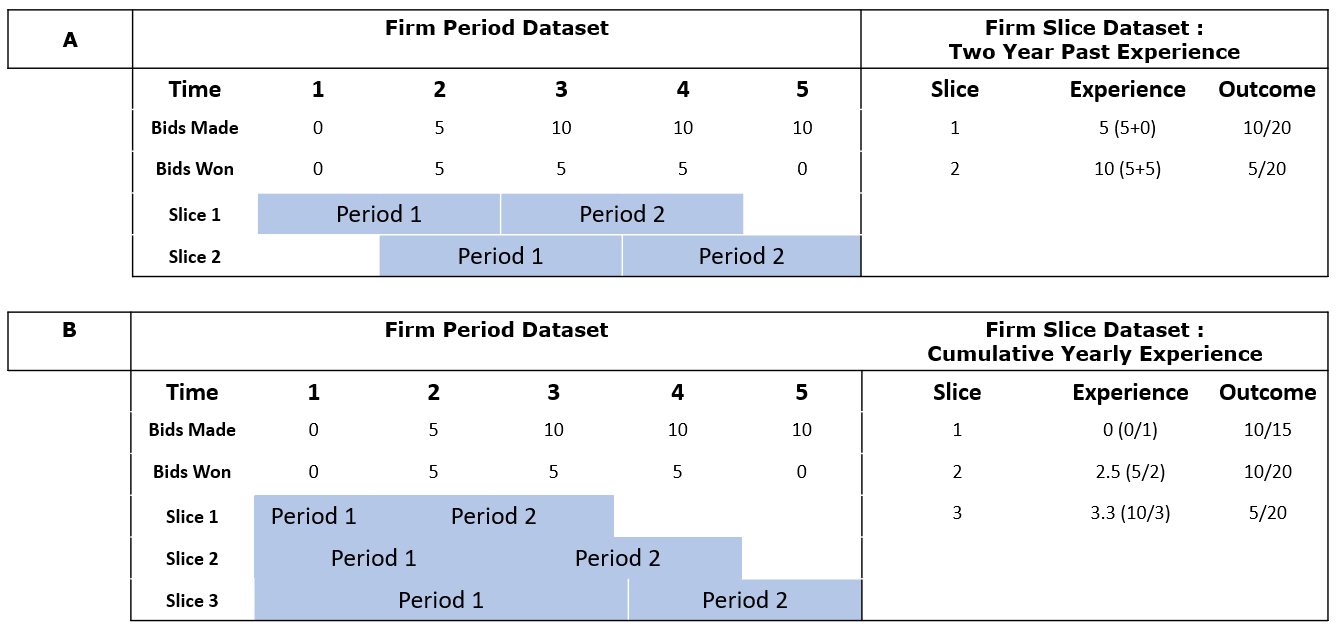
\includegraphics[scale=0.53]{diagram_experiences.png}
  \caption{Example computation of slice-firm dataset, employing two-year fixed periods of past experience (A), and cumulative yearly experience (B).}
  \label{fig:diagram_experience}
  \vskip 0.5mm
  { \footnotesize \underline{Note:} }
\end{figure}

%In some specifications we include firm fixed effects based on size. It is possible that smaller firms face higher competition due to less-complex contracts, and so their baseline level of success in the market will be lower.

After the transformation steps, we obtain ten slice-firm datasets for each measure of experience. Tables \ref{tab:slices_exp1} and \ref{tab:slices_exp2} show the amount of observations in each slice by the type of experience measure employed. Recall that every observation is a firm-level aggregate of past experience and summary of future outcomes and has the form of the rightmost table in Figure \ref{fig:diagram_experience}.

\input{C:/repos/learn-doing/thesis/tables/table_slices_exp1.txt}

\input{C:/repos/learn-doing/thesis/tables/table_slices_exp2.txt}


%The OLS regression in equation may have endogeneity problems. This next section discusses the sources of the problem and the identification strategy.


\subsection{Endogeneity and Identification}
We discuss two problems in the causal interpretation of equations \ref{eqn:olsspec1} and \ref{eqn:olsspec2}: endogeneity and heterogenous effects. We then present the empirical approach to identify consistently a feature of the distribution of treatment effects, the Local Average Treatment Effect.

First we discuss endogeneity. Unobserved cost variables, specific to each firm, are omitted in the OLS regressions above and expectedly endogenous. If there are highly efficient firms who are able to bid more aggressively or submit better proposals, they should win more projects, and in turn accumulate more experience over time. We thus expect our estimate $\hat{\beta},\hat{\gamma}$ in \ref{eqn:olsspec1} and \ref{eqn:olsspec2} to be biased upwards due to correlation (expectedly positive) between omitted cost variables and the amount of past experience.

To estimate consistently the treatment effect of experience on outcomes, we employ external variation to instrument the experience of a firm in an Instrumental Variables (IV) approach. We propose to employ close wins as an instrument for total wins (experience). If we are able to find wins where the success of a firm is less or not at all attributed to unobserved cost factors, or other efficiency advantages, but instead attributable to random differences (e.g. the conservativeness of each firms' engineers' estimates), we can estimate consistently the coefficient of interest by instrumenting total wins with close wins.

In this approach, our first stage takes the form of Equation \ref{eqn:firststage}. Here $EXP>0_{it1}^k$ is an indicator for contracts won in period 1 of slice $t$ for firm $i$, while $EXPCLOSE>0_{it1}$ is and indicator for a close win in the same period, and $\nu_{it}$ is an error term uncorrelated with $EXPCLOSE_{it}$. The second stage is shown in Equation \ref{eqn:secondstage}.

\begin{equation}
\label{eqn:firststage}
EXP_{it2}>0= \delta EXPCLOSE_{it}>0+T_t+\nu_{it}
\end{equation}

\begin{equation}
\label{eqn:secondstage}
S_{it2}= \beta EXP_{it2}>0+T_t+\varepsilon_{it}
\end{equation}

Both measures of experience ($EXP$ and $EXPCLOSE$) should be correlated since every extra unit of experience increases the probability of having at least one close win, fulfilling this way the rank condition. Moreover, close wins should not be correlated with cost measures, as they are attributed to random factors, such as risk-aversion differences between firms, random approximation differences between engineering teams in each firm, etc. and thus ensuring a valid instrument as well.

Even tough our estimate $\hat{\beta}$ is consistent,
we do not expect to identify the a single Treatment Effect because treatment effects should be heterogenous:
\begin{itemize}[itemsep=1pt]
  \item Experience itself is heterogenous given the complexity, length and size of a project, so it is expected that treatment effects are also heterogenous.
  \item Firm's absorptive capacity and learning ability depends on internal skill, financial strength and other organizational variables.
  \item More experienced firms should see diminishing returns to experience.
  \end{itemize}

 Following the discussion of \parencite{angrist1995identification} as presented in \parencite{hansen2009econometrics}, we argue that the estimation strategy identifies the Local Average Treatment Effect for our binary treatment, i.e. $EXP>0$., i.e. the average treatment effect for the firms that are affected by the experience treatment if and only if they win a contract by chance (i.e. “compliers”). This interpretation, additionally to rank and validity, also requires a monotonicity condition, that here is equivalent to having no firms negatively impacted in their experience by experiencing a close win. This condition is satisfied in our setting, since a close win belongs by construction to the set of all wins.

Having discussed the theoretical rationale and identification for the instrument of close wins, the problem remains of how to successfully find close wins and label them as such, which is the purpose of the next sections. Two alternatives are proposed: first, find contracts with very close wins where price was heavily weighted, and second, develop a ranking measure of firms to find "balanced" auctions. Both are discussed and analyzed in the next sections.

\subsection{Definition of a close win}
We discuss what would be the optimal way of finding close wins, and, since the data does not allow us to employ this strategy, we propose two second-best alternatives.
The optimal way to identify close wins would be to single out auctions for which the winning firm had a final weighted score which was marginally superior to the ones of its competitors.  Recall that, for each contract, the  proposals from firms are scored in several criteria, weighted, and finally summed to produce the total score for that firm. Unfortunately, the previous strategy is unfeasible with the data we have available. Our data only allows us to see the criteria employed in each contract and the weight of each factor, but not the individual scores for each firm. We attempt two alternative methods detailed in the subsections below.

\subsubsection{Close wins by price}
In this method, close wins are operationally identified as the wins where i) the winning bid  was not more than .05\% below the second lowest win, if he had the lowest bid, ii) the winning bid  was not more than 0.05\% below the lowest bid, if he did not submit the lowest bid and iii) the weight of the price item in the awarding decision is more than 50\%.copulatively  two conditions: i) the price weight in the awarding decision criteria is 50\% or higher and ii) the difference between the lowest bid and the second lowest bid is less than .05\%. This way of identifying close wins should indeed capture a subset of the random wins, namely, random wins in projects where price is the major awarding criteria.

This definition of close wins leads to approximately 2\% of winning bids being classified as a close one. In Table \ref{tab:closewins_alt1_desc} we examine whether close wins defined as above are different from the population in several types of metrics. We can see that in most aspects these bids have less dispersion in variables such as participants and less size. These might because of fat tails in the distributions of sizes and participants.

\input{C:/repos/learn-doing/thesis/tables/table_closewins_alt1_desc.txt}

The rank condition is verified via a regression of experience on close experience. The F-Statistic of this regression is 118.2 for the indicator treatment and 1,500 for the continuous measure.

\subsubsection{Close wins by rank}
%There coul two main objections to the previous identification strategy:
%\begin{itemize}
  %\item The price is not the only awarding factor. Thus, it is possible that even in a contract where price is a major component, the cost advantages of a firm manifest in terms of other awarding factor, like quality. That is, the firm offers similarly priced goods but at a much superior quality.
%  \item The closeness between the first and the second bid does not take into account the full pool of participants.
%\end{itemize}

The second strategy to identify close wins does not rely in prices or any other aspect of the bid itself. Instead, we label a winning bid as a close win if all the firms involved in the auction were close in ranking. The argument here is that, given a well constructed ranking, winning a contract against closely placed opponents should be attributable to random factors.

Obviously, the main issue is how to construct a good ranking measure. We proceed by  modeling each auction as a multi-player game event (in the non-economic sense of the term) in which firms gain points by winning the project and lose points by not winning it. We award and subtract points based on a modified ELO algorithm suited for multi-player games.

Each firm has its ranking initialized at a pre-specified level (1,500 in the initial version). Then, it is awarded 25 points for winning against a similar opponent and subtracted 8 by losing. The implementation of the algorithm recommends that points awarded and subtracted sum to zero, so we fix awarded points and choose subtracted points so that on average (given the number of players in an auction) this condition holds. Against non-similar opponents, the algorithm makes a correction on points awarded and subtracted based on the ranking of the players and the outcome of the game.

Proceeding from the oldest to the most recent auction, we update the initial rankings for each firm and obtain for each firm its ranking at any point in time. Next, we label a win as a "close win" when the highest rank among the bidders for the auction was not more than 3\% higher than the lowest rank among the same set of bidders. This yields around  5,800 closely won contracts (11\% of the contracts in the analysis sample) which corresponds to 17,000 observations (11\% of the observations in the analysis sample). In Table \ref{tab:closewins_alt2_desc} we present summary statistics for close wins identified via rank.

\input{C:/repos/learn-doing/thesis/tables/table_closewins_alt2_desc.txt}

In the analysis, we drop the first year of data to allow for a period of rank adjustment. This is necessary since the algorithm does not work well when the average rank in the population is not clearly defined. The way ranks evolve as time progresses  can be seen in Figure \ref{fig:rankings_times}. Note that ranks appear highly concentrated at the end of the first year of data, while they are much more dispersed at the end. In the robustness checks we analyze both i) different values for the won/lost points after an auction and ii) the threshold in ranking for a close win.

\begin{figure}
  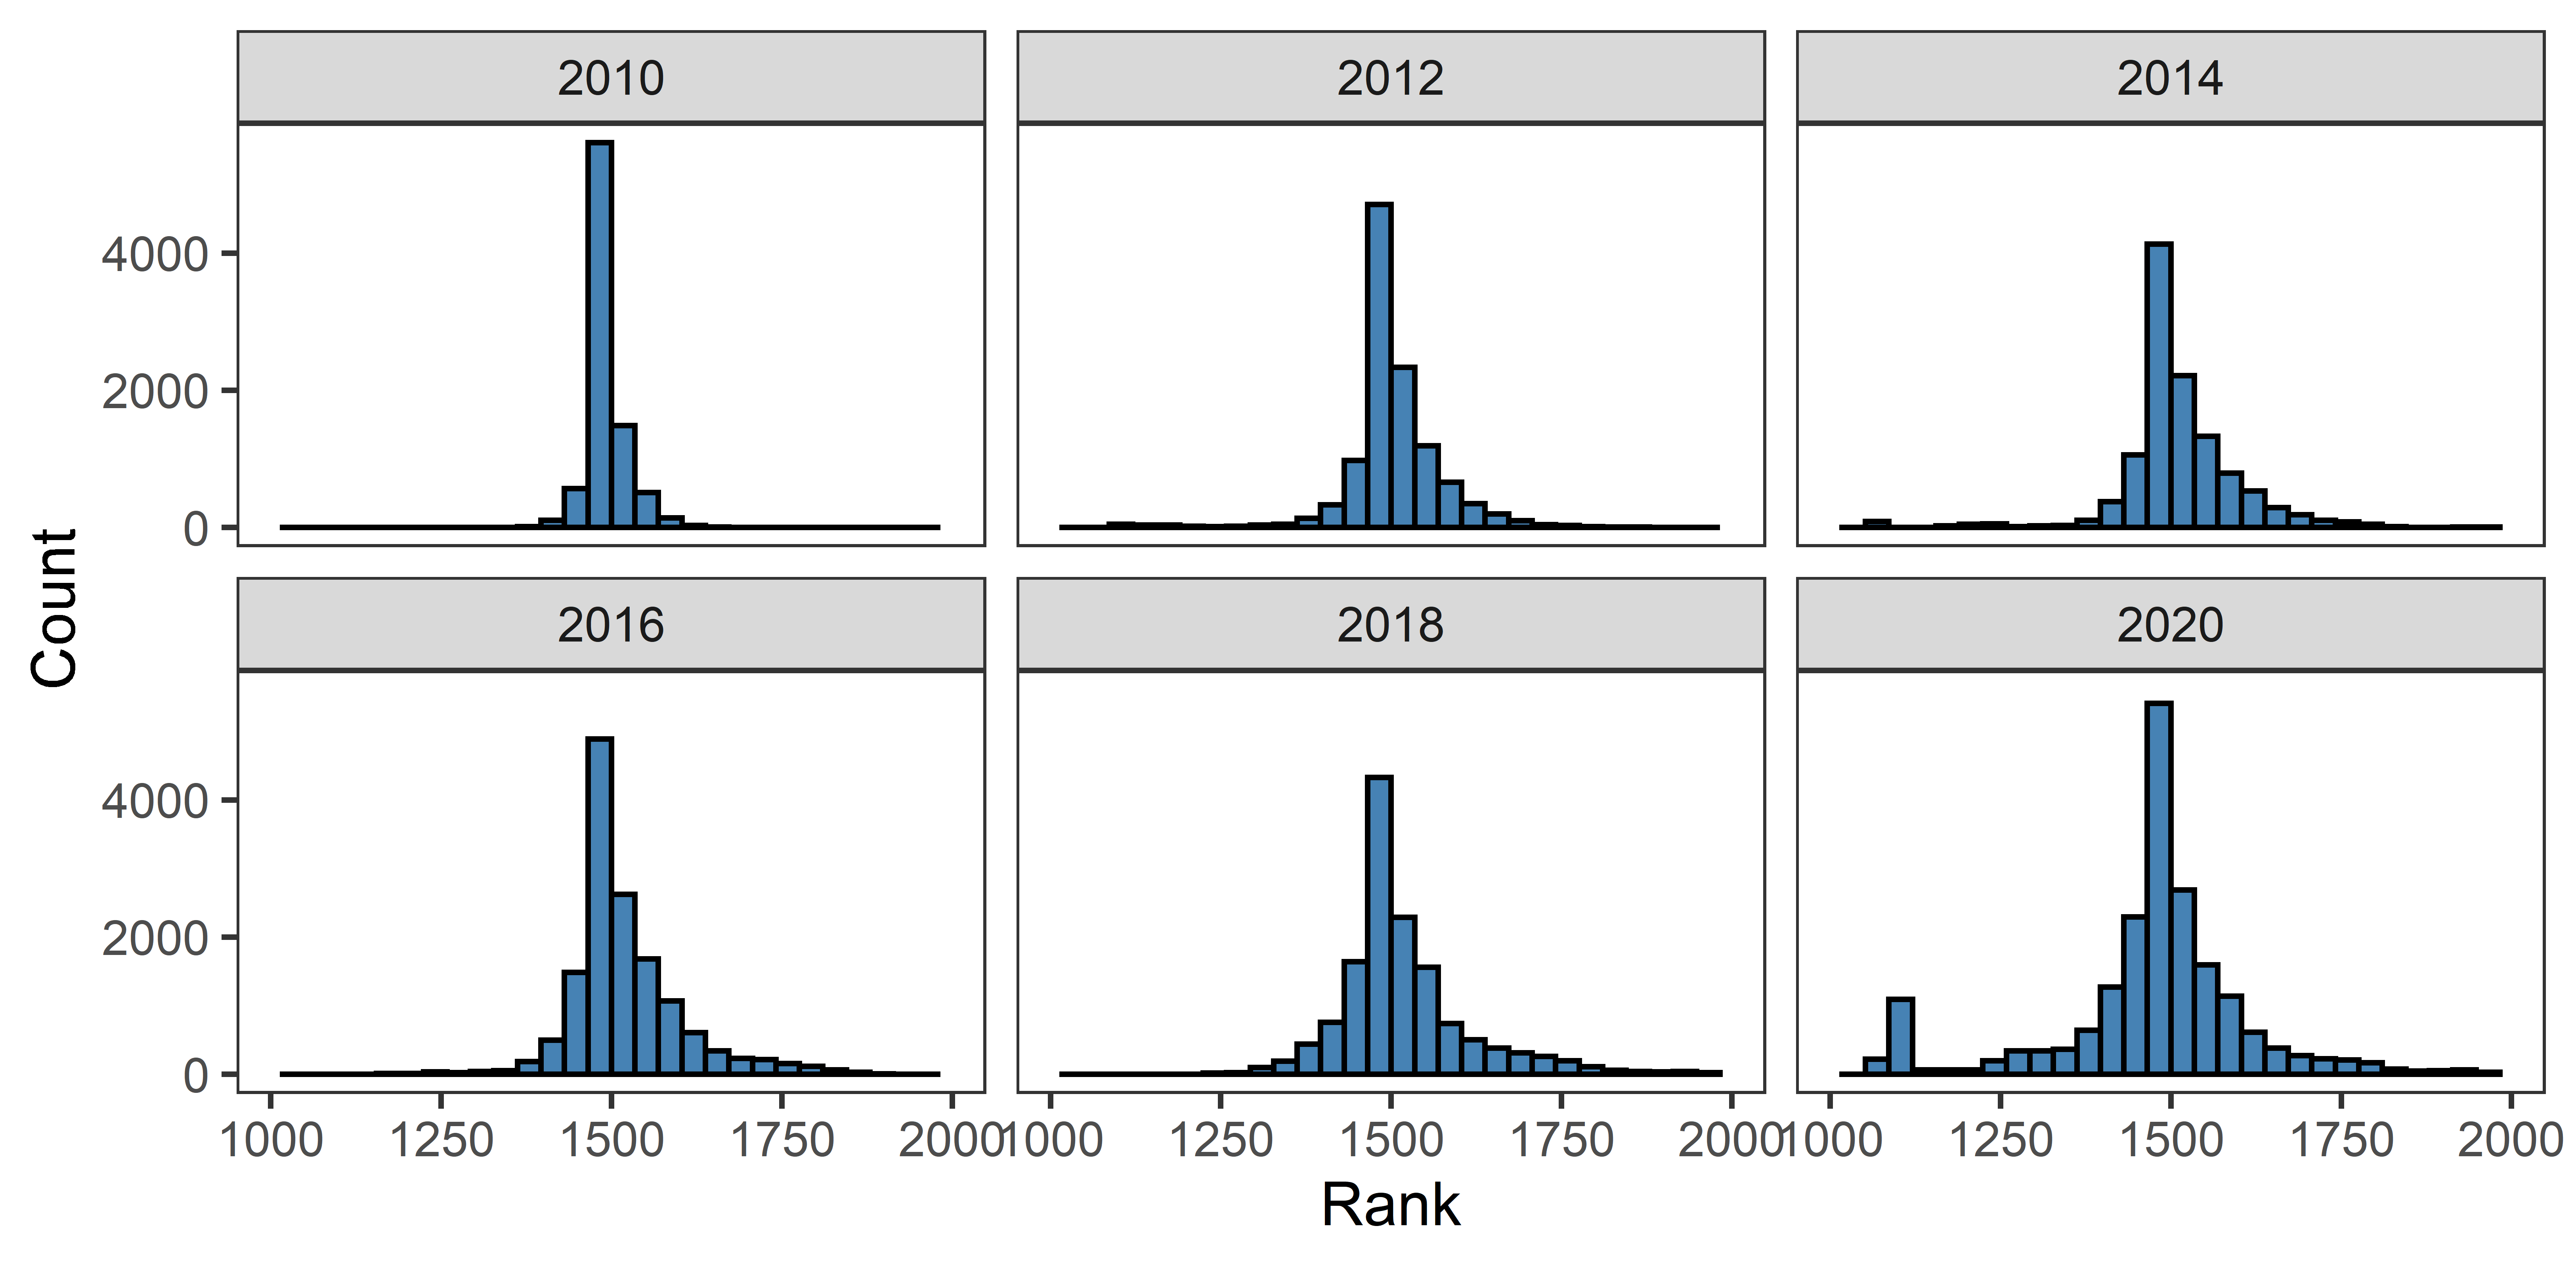
\includegraphics[scale=0.90]{rankings_times}
  \caption{Evolution of ranks by selected years}
  \label{fig:rankings_times}
  \vskip 0.5mm
  { \footnotesize \underline{ } \par}
\end{figure}


\clearpage
%Bidding behavior
%An alternative way to measure changes in bidding behavior caused by efficiency gains through experience is to examine directly changes in bidding behavior among more experienced firms with respect to less experienced ones. As was discussed before, experience induces changes in the underlying production function, or changes along the production function, that make the firm more efficient at producing certain types of goods. In a competitive market, firms should pass through at least a fraction of this improvement in costs to the bids they submit in the auctions. Thus, we should be able to identify this change directly through the bids that more experienced firms submit for projects.
%The approach is different than the one from the previous section because we can directly link the past experience of a firm to each bid it submits in every auction that it participates in. Thus, our unit of observation is a bid submitted by a firm for a contract of a public construction contract. Our second specification has then the following form:where is the standardized bid submitted by the firm and is a measure of past experience. In further specifications we include a broader set of controls. First, we add fixed effects by auction. Second, we add firm fixed effects. Finally, we control by the geographic region where the auction is being held.
%The outcome variable is the standardized bid submitted by firm to the auction, i.e. the original bid amount divided by the engineering estimate of the project. This approach allows us to make comparisons along project of different sizes. It is also useful because it should be expected that our dependent variables have effects per unit of contract amount (Bajari, 2010). The standardization also controls for some sources of heterogeneity.
%The dependent variable is the total number of contracts that the firm has won up until the moment that the firm submits its bid. Since for the first periods in the data we do not have information on past experience, we exclude the first two years from our observations of outcomes and only employ them to compute experiences for firms from year three and onward. In the robustness section, we explore several alternative ways to measure experience and subset the set of firms.
%In the same way as before, we expect that there will an endogeneity between cost measures and bidding behavior. We should expect that firms which have a baseline efficiency higher than other firms will be able to submit lower bids and gain more experience, so we could pick up effects of reverse causation in our coefficient for experience.  We thus employ a similar Instrumental Variables approach as before, instrumenting total past contract wins with close contract wins.

\section{Main Results}

First we explore graphically the relationship between experience and outcomes. Figure \ref{fig:plotresults_both} shows the relationship between rolling (top row) and annualized (bottom row) measures of experience and outcomes.  Each column represents a different subsample and dependent variable. The first column (panels A and D) selects all firms and displays past experience in the $x$-axis. The second column (panels B and E) contains only firms with equal experience and close experience (including zero). The $x$-axis displays the close wins. The third column (panels C and F) is analogous to column two but employs the definition of a close win as close win by firm rank.

We observe that average winning shares increase with more experience. The effect appears to be close to linear, although for experiences higher than ten contracts performed (rolling) or five contracts performed (annualized) we have wide error bars or no observations available. In the case of our "reduced form" graphs, we observe that almost always the close wins seem to improve average winning shares, although we observe wide error bars in the second column, caused by the low amount of observations that fulfill the conditions imposed.

Next we show the results from our regression analysis. Table \ref{tab:table_exp_1} shows the results for OLS and IV regressions for our first experience measure (i.e. rolling two year periods) while Table \ref{tab:table_exp_2} shows the results for our second measure of experience (i.e. annualized experience). The first three panels in each table employ as treatment the binary indicator of experience, whereas the last three panels employ total experience.

The OLS estimate of the effect of having experience on winning proportion is 0.07 for rolling experience and 0.06 for annualized experience. IV estimates of the coefficient are very close to OLS counterparts or even higher, for the case of annualized experience. The specification with linear returns on experience shows that experience renders a 0.01 and 0.03 increase in winning share per extra contract developed (for rolling and annualized experience respectively). IV estimates of linear effect of experience are again close to OLS counterparts. Finally, almost all the estimates for the experience treatments are significant at $p=0.01$ with robust standard errors.

A concerning result is the low $R^2$ of the regressions, which shows that although the effect of experience on the mean outcome is significant, there is much variability among firms' outcomes which is not explained by the increase in experience.

Given the average winning shares (0.2), the effect of having experience is equivalent to an increase of almost 30\% of the winning share of a firm (i.e. around 7 percentage points out of 21 percentage points). This points towards significant importance of previous experience in future outcomes.

%Altough initially we intended to show results regarding a quadratic term on experience, exploratory results showed that there was almost no difference with employing a linear term so we omitted these specifications in the main results.

\begin{figure}
  \includegraphics[scale=0.6]{plotwins_panel.png}
  \caption{Relationship between contracts won on $t-1$ and mean winning probability across contractors in $t$.}
  \label{fig:plotresults_both}
  \vskip 0.5mm
  { \footnotesize \underline{Note:} The plots show the mean across firms of the number of contracts won out of the number of contracts bid for in period $t$ (in the $y$-axis), against experience accrued in period $(t-1)$ in the $x$-axis. $t$ and $t-1$ correspond to two periods of two years each for the top row, for the bottom row $t$ is also a period of two years, but $t-1$ are all years in the interval $[2010,t]$. Error bars correspond to means plus/minus two standard errors. First column: all sample observations are considered. Second column: only contractors with experience = close experience. Third column: analogous to second column employing the rank definition of close win.  The rirst row definition of experience is rolling experience while second row employs cumulative annualized experience.\par}
\end{figure}
\clearpage

\input{C:/repos/learn-doing/thesis/tables/table_ols_exp1.txt}

\input{C:/repos/learn-doing/thesis/tables/table_ols_exp2.txt}

\clearpage

\subsection{Comparing with contracts that do include experience in awarding score}

We compare the main results obtained in the previous section with the results obtained by considering for outcome computation only contracts which $do$ require experience in the awarding criteria. This helps to put the results in context and also serves as a validation check of the empirical strategy. We expect to find greater estimates for the effect of experience on outcomes among contracts which explicitly reward experience.

Figure \ref{fig:comparison_considers_experience} shows the estimate from the IV specifications, both with linear and binary functional forms of experience, by the type of contract considered to compute outcomes (we only employed rolling experience). It can be seen that the effect of experience on outcomes is about twice as big in contracts which do consider experience as a factor in the awarding criteria with respect to those who do not.

\begin{figure}[H]
  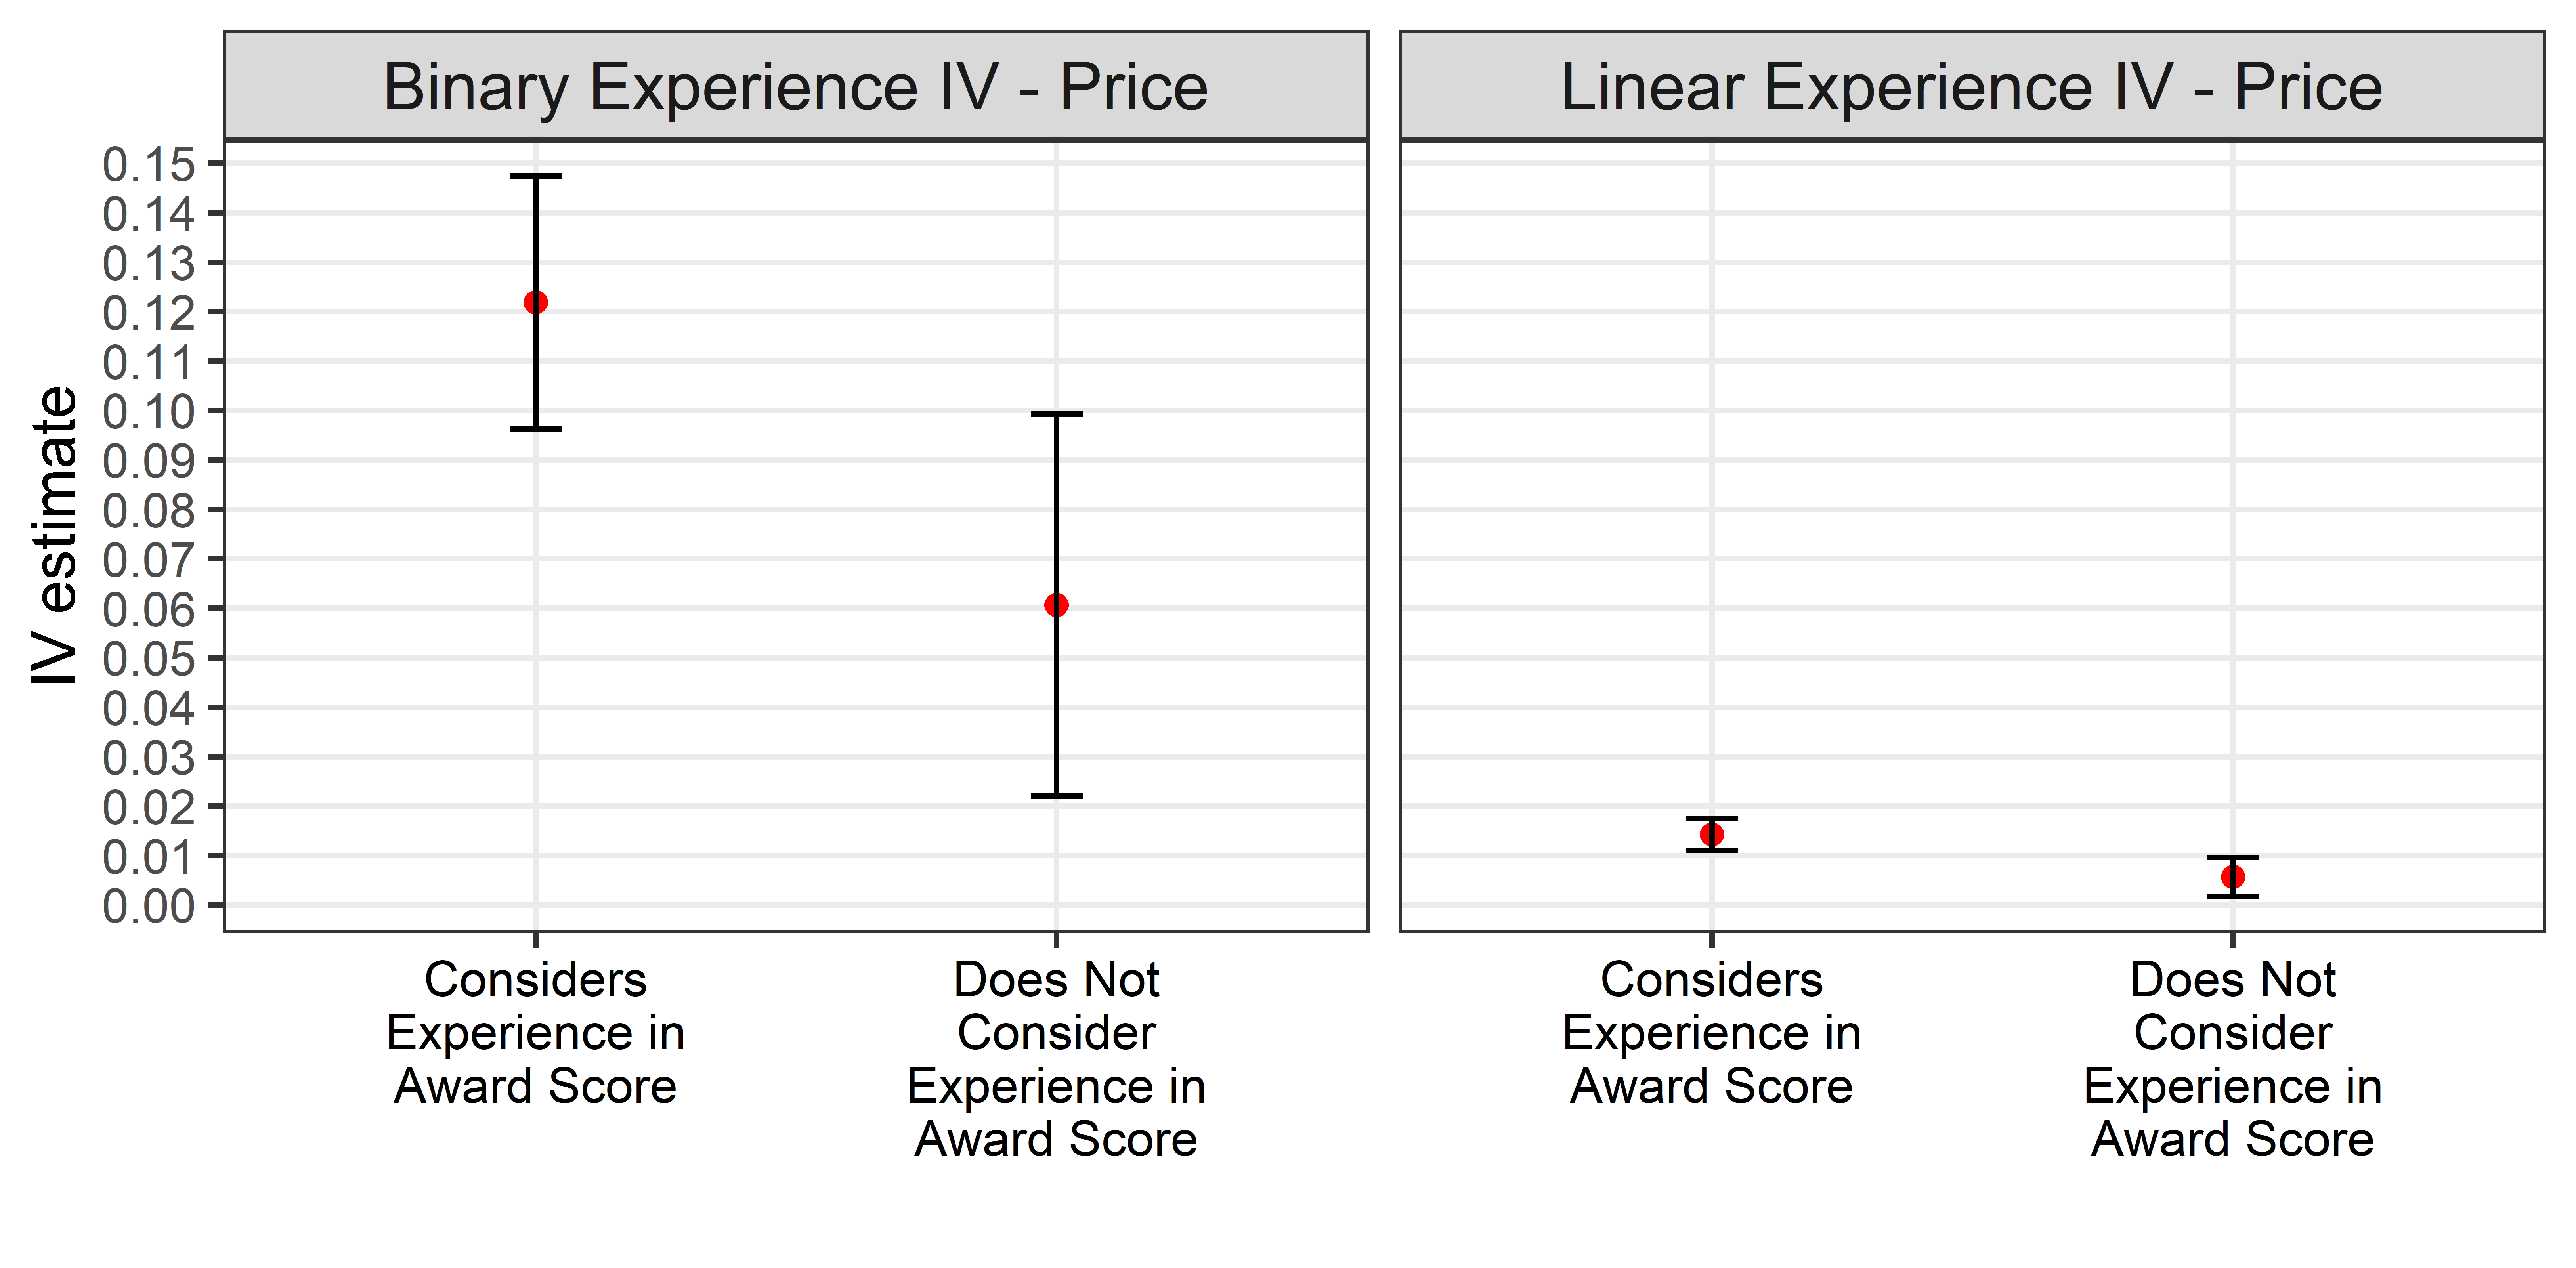
\includegraphics[scale=0.9]{comparison_considers_experience.png}
  \caption{Comparison between estimates obtained in contracts with and without experience in the awarding criteria employed by the government}
  \label{fig:comparison_considers_experience}
\end{figure}

%There does not seems to be conclusive evidence regarding different results when employing quadratic rather than linear functional forms for experience. For example, Figure \ref{fig:pred_average} shows the mean confidence intervals, employing as period fixed effects the last period in the sample. It can be seen that the fitted total predicted value does not seen to vary greatly from the linear to the quadratic specification.

%\begin{figure}[H]
%        \centering
  %      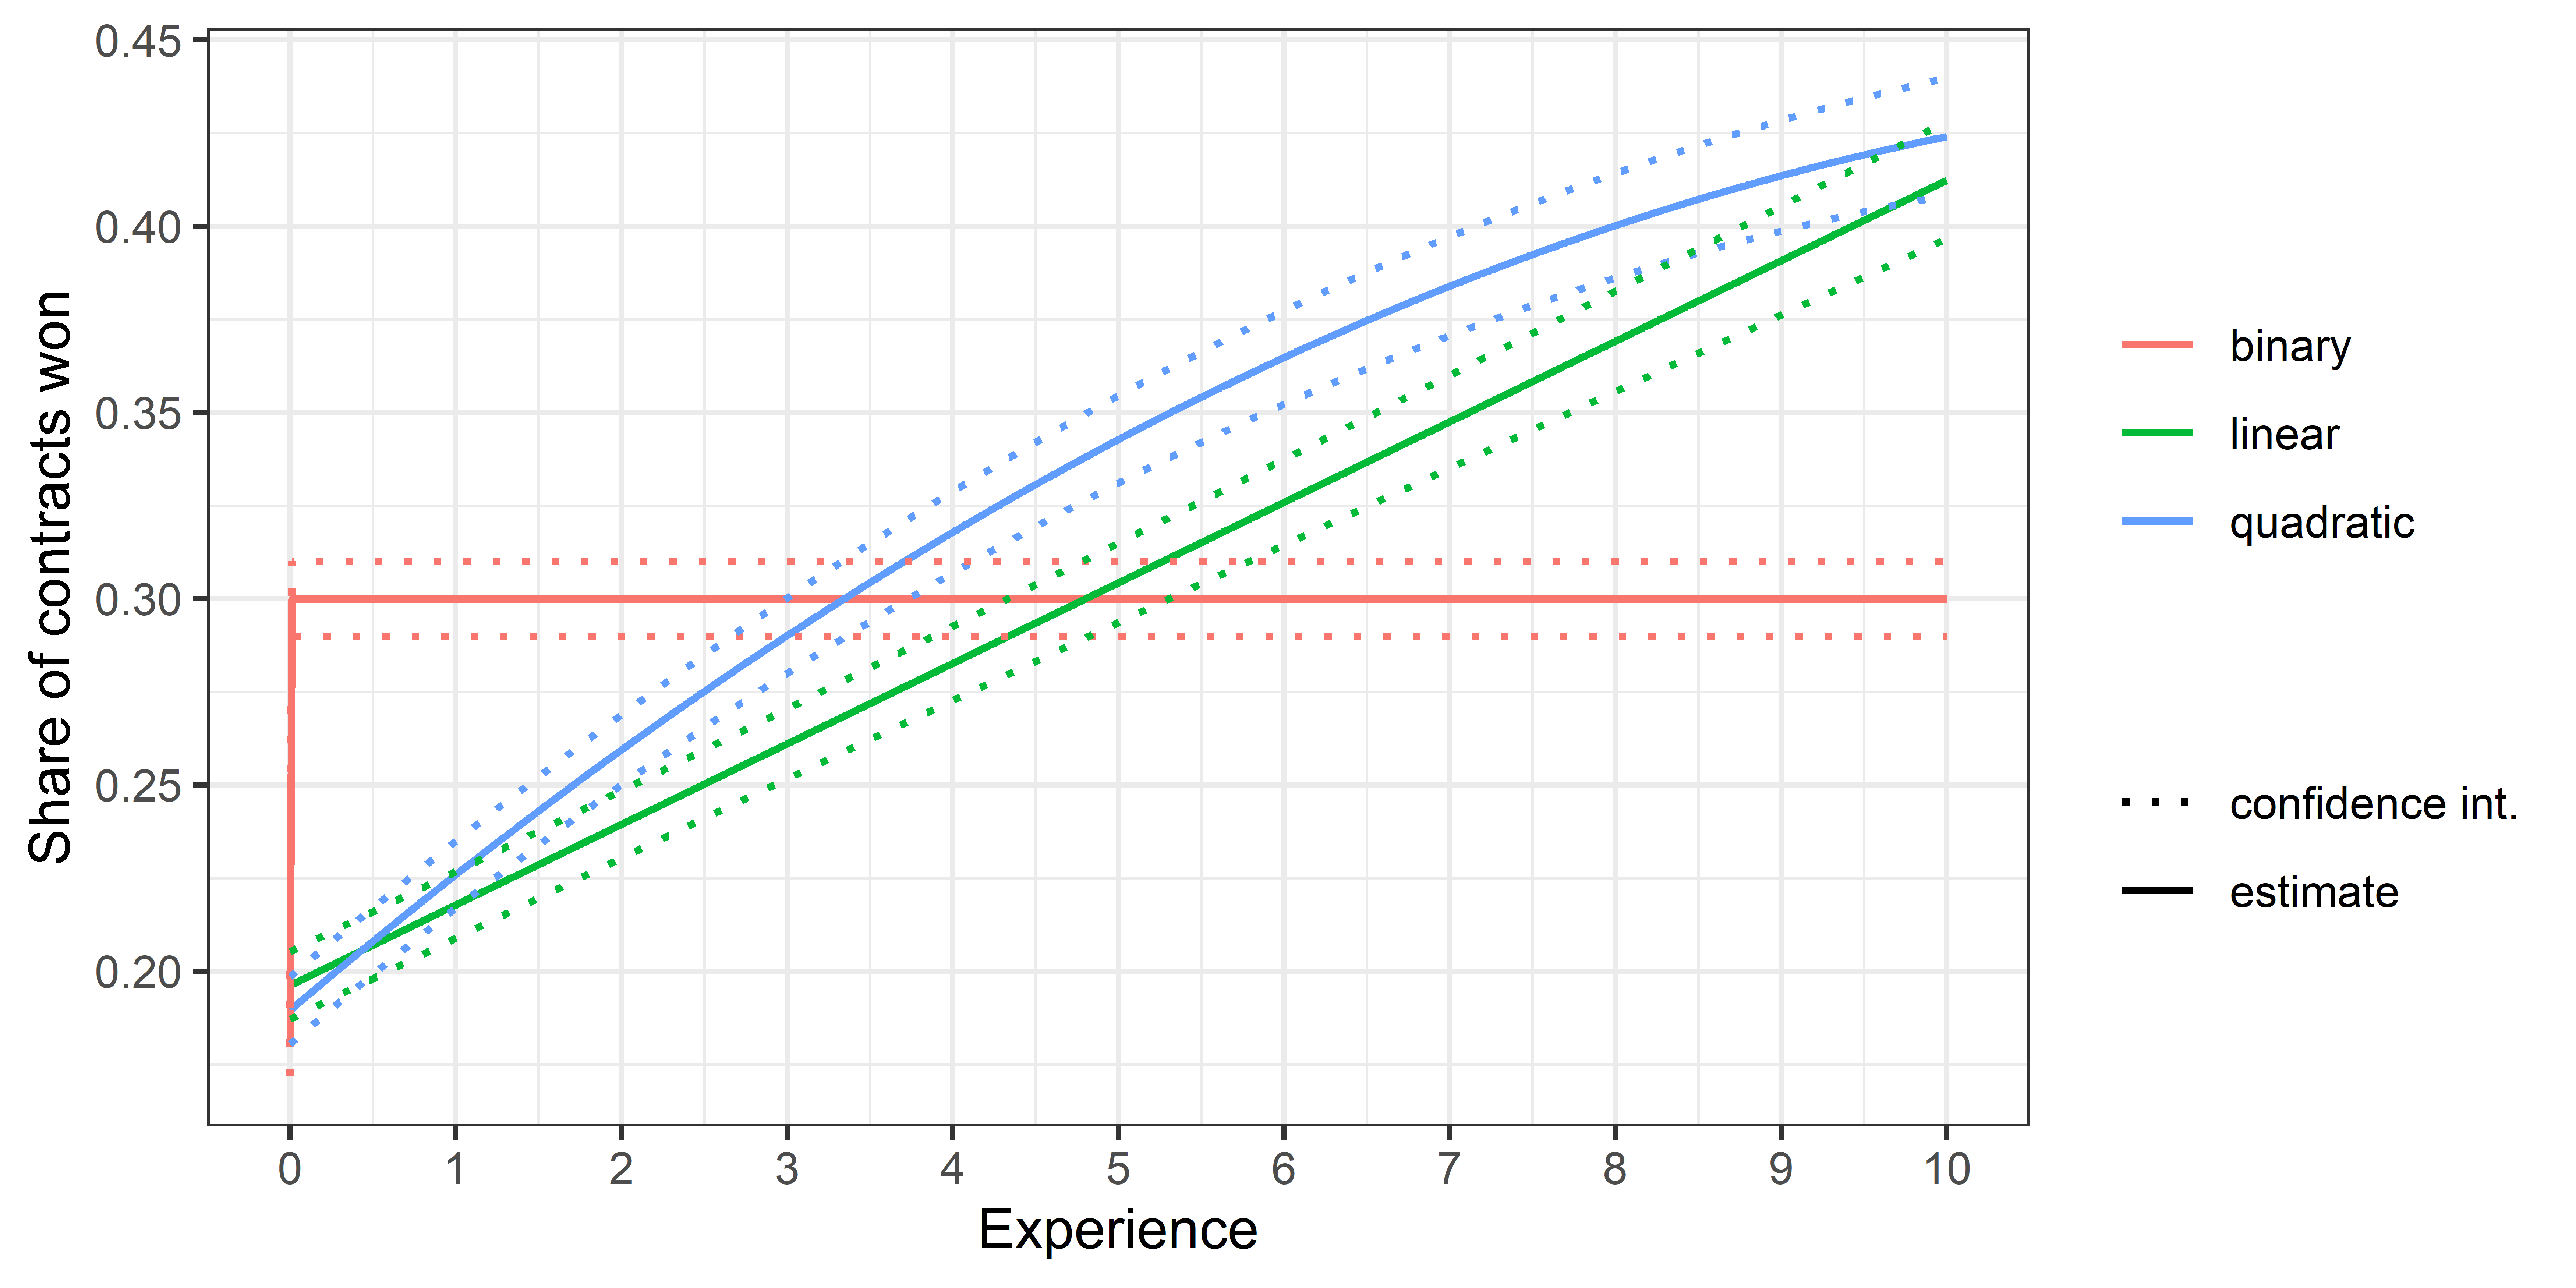
\includegraphics[scale=0.8]{fit_sample.png}
  %      \caption{ \small Predicted values for the mean of the outcome variable (share of contracts won), by total experience accrued in the previous period. We employ fixed effects as in the last period of the dataset.}
  %      \label{fig:pred_average}
  %  \end{figure}

%\begin{figure}
%  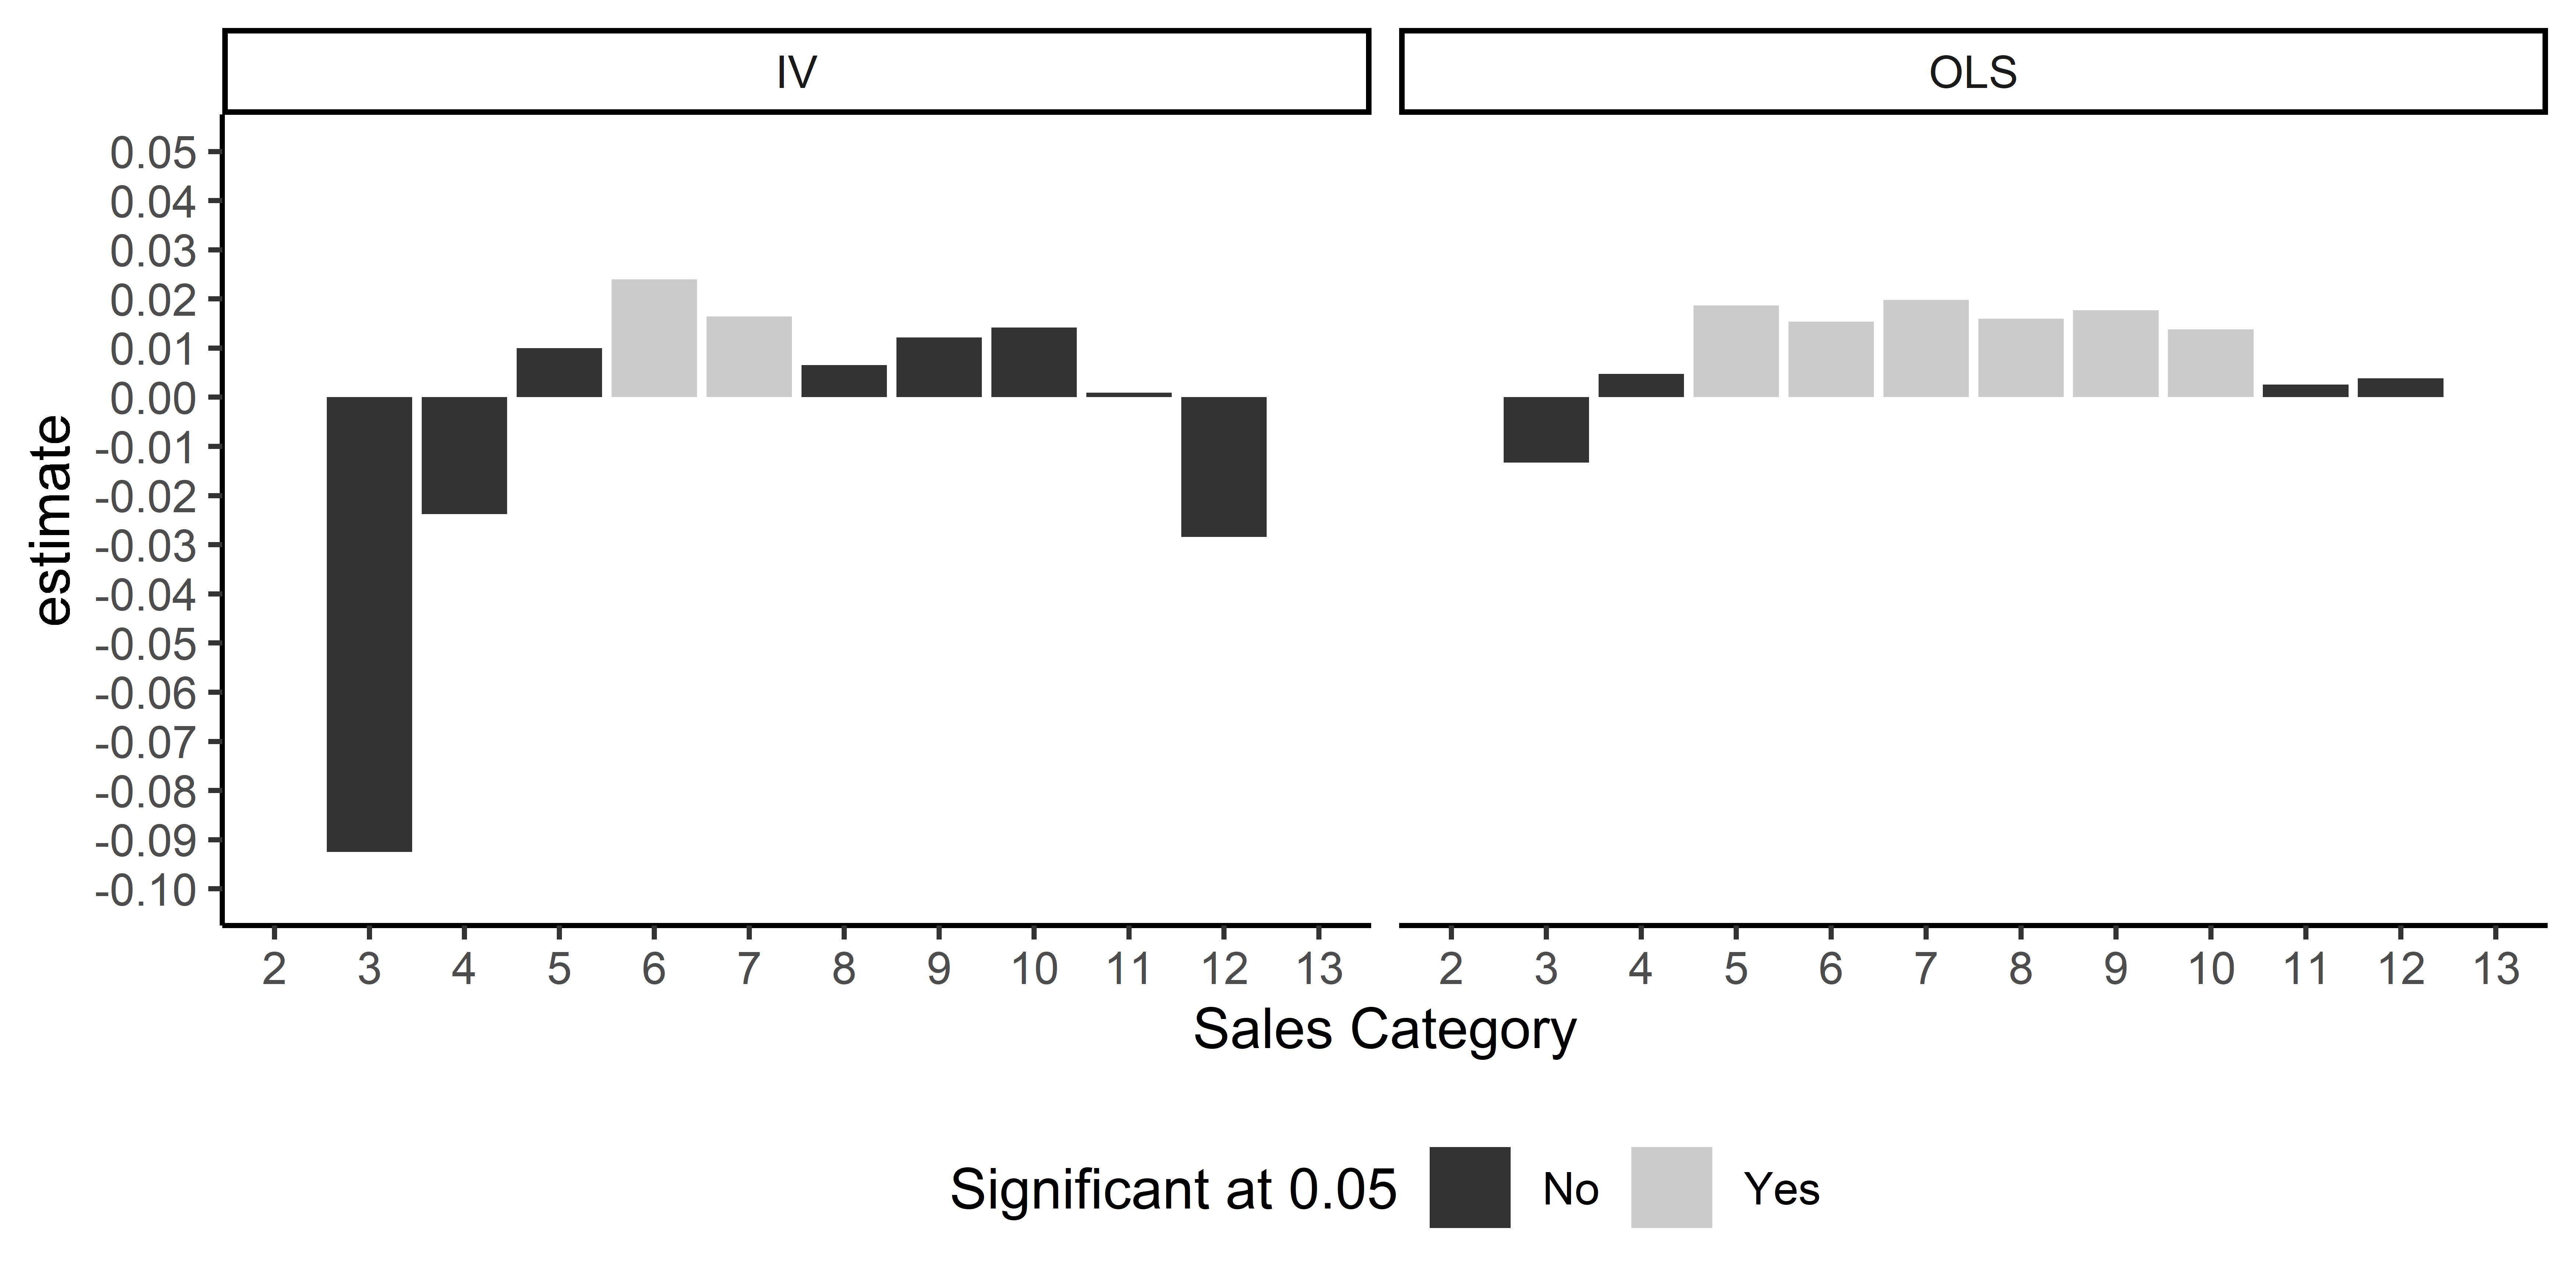
\includegraphics[scale=0.85]{plotsize.png}
%  \caption{Experience coefficient by tax sales category}
%  \label{fig:sizeestimates}
%\end{figure}

%\resizebox{\textwidth}{!}{%
%\input{C:/repos/learn-doing/thesis/tables/table_sizes_explinear1.txt}
%}%


\section{Robustness checks}
Several of the parameters in the empirical strategy of the previous section admit more than one reasonable choice. This section considers alternatives for them. Robustness checks are studied for the following parameters:
\begin{enumerate}
  \item Periods of outcome computation.
  \item Definition of a close win (by price).
  \item Definition of a close win (by rank).
\end{enumerate}
\subsection{Periods of outcomes}
In the main analysis, we computed outcomes across a period of two years for each of our slices. This choice is sensibilized by computing outcomes in one and three year periods as well. While varying the length of the period where outcomes are computed, the procedures to compute experience are kept the same as before.

A shorter timeframe would be a better parameter choice if: firms bid frequently, so their true outcomes manifest quickly;  learning is itself instantaneous,  so past experience immediately influences outcomes; or  the learning effect is short lived, which would make much more important for the outcomes the recent history. Conversely, a longer time frame is better in the case of infrequent bidding, slow learning, and long lasting knowledge.

For construction projects, it is expected that the better parameter would be more close to a longer timeframe than to a shorter one. Construction projects, especially complex ones, can be less frequently auctioned than in simpler, undifferentiated products. More importantly, since construction projects take longer to perform than regular purchases, it is reasonable to expect a longer learning process.

Table \ref{tab:robust_bin_outcomes} shows estimated experience coefficients where outcomes were computed in periods of 1, 2 (the original specification) and 3 years. The rows correspond to OLS, IV (by price) and IV (by rank) specifications. Notably, i) all results are significant with $p<0.01$ and ii) estimates are close to each other across different values of the parameter. Standard errors decrease with the number of years considered because of the increase in sample size. In almost every case, estimates remain within a standard error of the original estimates, and in all cases they remain within two standard errors.
\input{C:/repos/learn-doing/thesis/tables/robust_bin_outcomes.txt}

\subsection{Definition of a close win - Price IVs}
In the main section, close wins by price were defined as those in which the winning contractor submitted a bid that i) was not more than .05\% below the second lowest win, if he had the lowest bid, ii) was not more than 0.05\% below the lowest bid, if he did not submit the lowest bid and iii) the weight of the price item in the awarding decision is more than 50\%. In this section the main estimates are sensibilized to different values of the threshold parameter and the weight parameter.

We first sensibilize the threshold for bid differences for the linear estimate of experience in the rolling experience measure. The plot in Figure \ref{fig:close_wins_robust} displays the coefficient of interest and 95\% confidence as we vary the threshold for a close win.  For thresholds below .25\%, we obtain much wider standard errors. The reduction in sample size for the instrument is significant below .5\%, since this percentage is already at around the 15th percentile of bid differences in the sample. However, we keep significant outcomes at p=0.05 for all values analyzed.

 \begin{figure}[H]
         \centering
         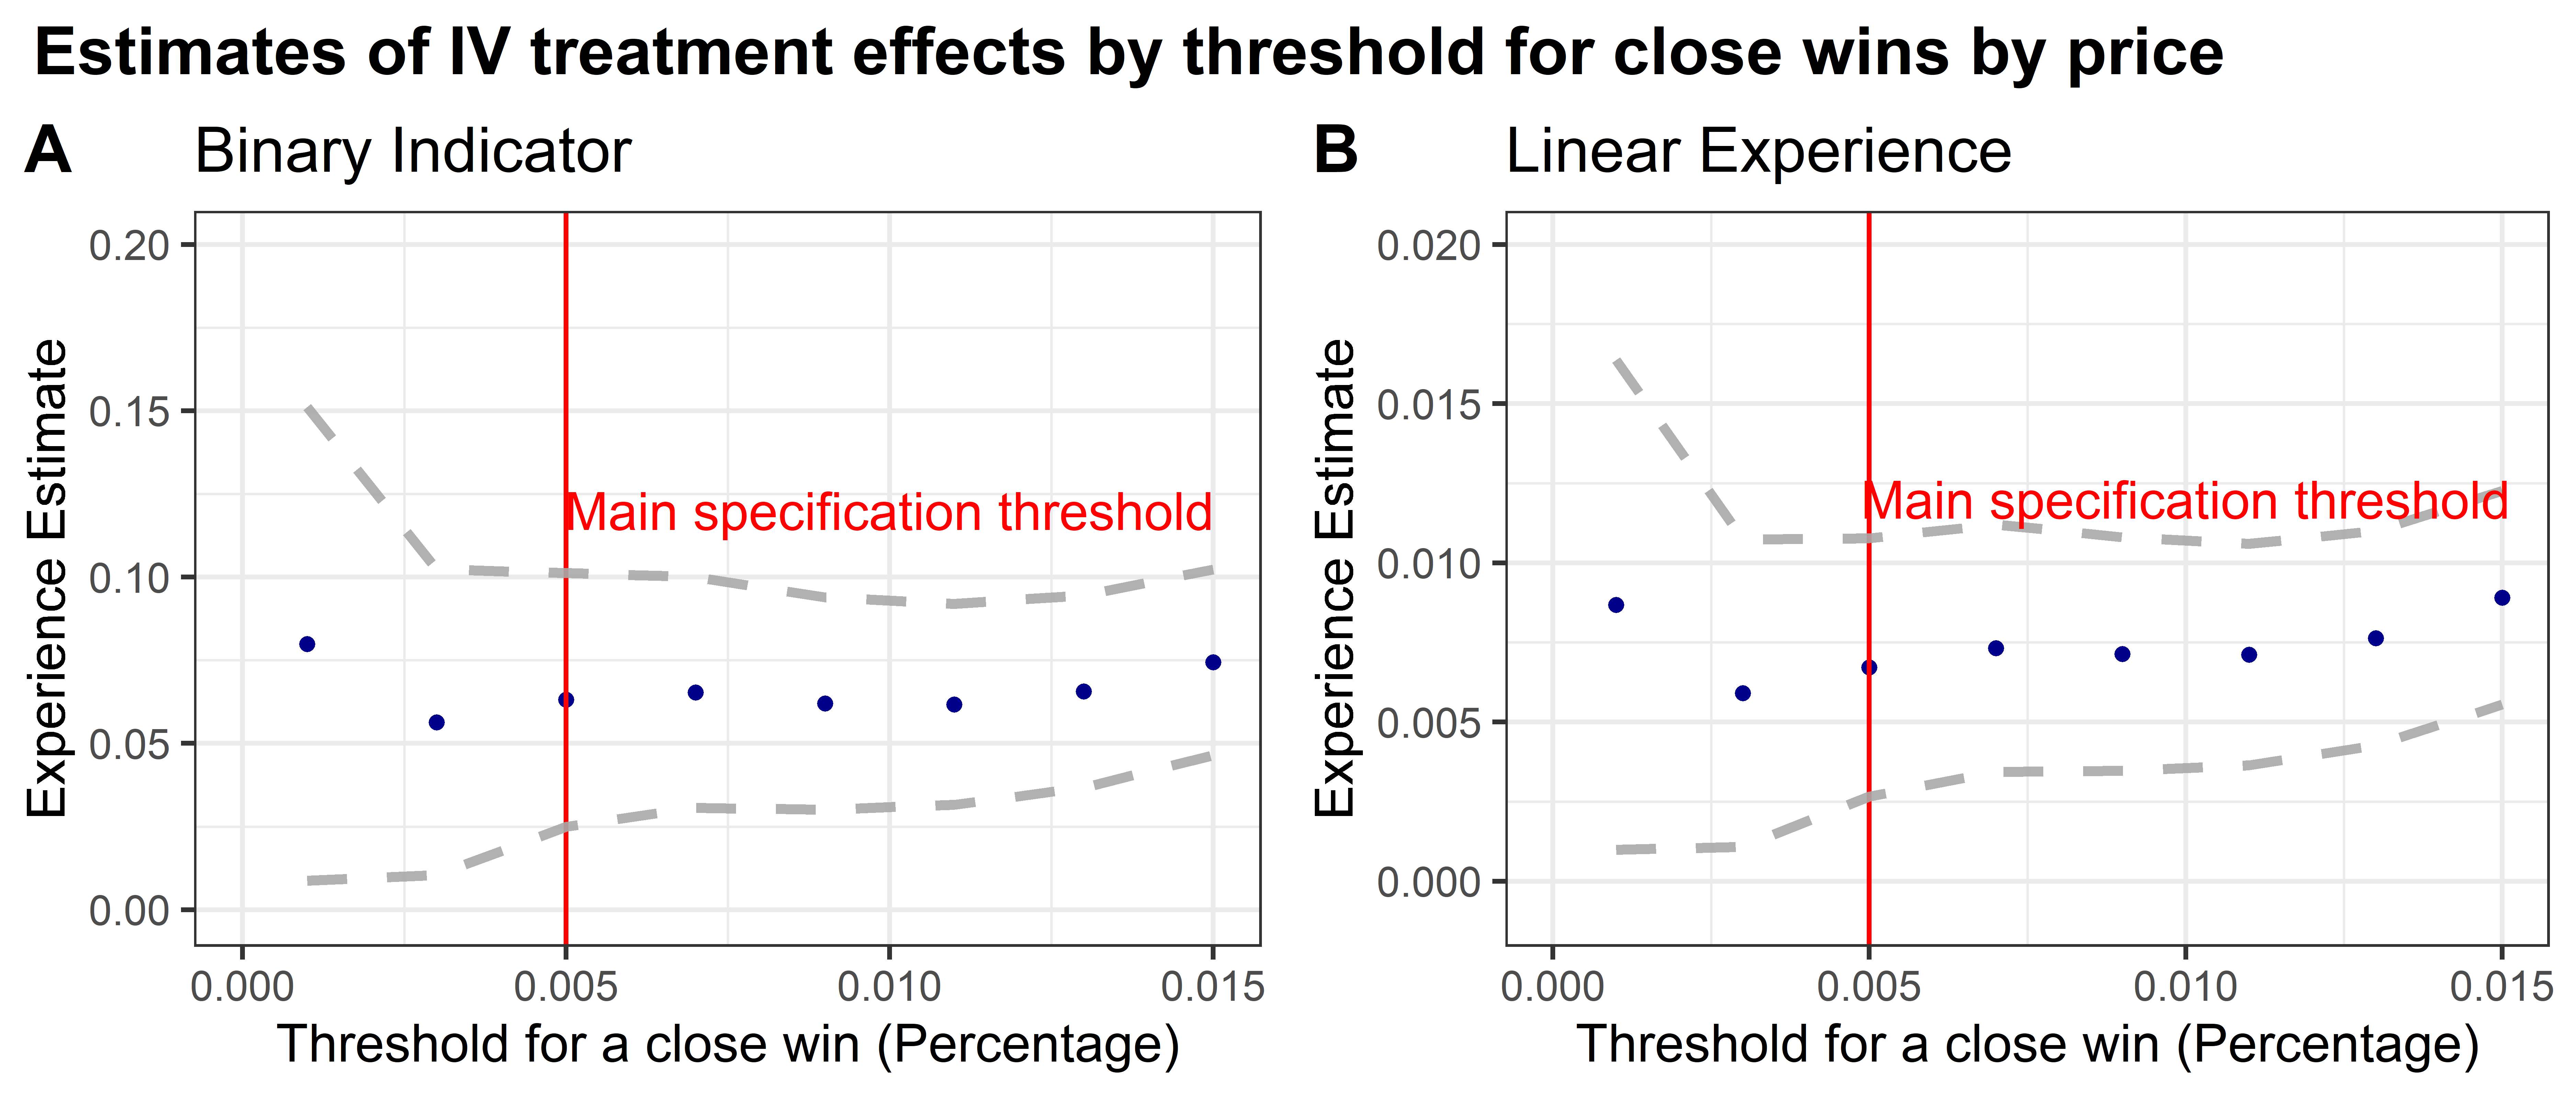
\includegraphics[scale=0.85]{robustness_threshold.png}
         \caption{Robustness analysis for threshold of close wins}
         \label{fig:close_wins_robust}

  \vskip 0.5mm
  {\justifying\footnotesize\underline{Note:} The plot shows the coefficient on experience as in the specification of Panels 4 (left) and 5 (right) of table \ref{tab:table_exp_1}, that is, the dependent variable is the share of contracts won in period $t$ and the independent variable is an indicator of experience or linear experience. Experience is instrumented with close wins in period $(t-1)$. The $x$-axis shows how the coefficient varies with the threshold for what is considered a close win.\par}
 \end{figure}

Next we examine the parameter for the weight of the price component in the total score. We replicate our main IV-price results but consider weights  of 60\%, 70\%, and 80\% as the minimum weights of the price component in the factors considered to evaluate proposals. Table \ref{tab:robust_weightprice_outcomes} shows the results. At 60\%, most results remain significant, but beyond 70\% almost all results are not. Since 60\% is the 80th percentile of the score weight across contracts, we have again a sample size problem for the instrument when there are higher requirements for the threshold of the price weight.

\input{C:/repos/learn-doing/thesis/tables/robust_weightprice_outcomes.txt}

\subsection{Definition of a close win - Rank IVs}
The IV-Rank estimates are sensibilized by choosing alternative thresholds for the maximum difference between the highest and lowest bidder's rank (bandwidth) and different values for the points awarded for a win. Recall that an auction is labeled as close in the main specification if the difference in rank between the highest and lowest ranked in the auction is less than 3\%. In the main specifications, 25 points are awarded for a win and eight are subtracted for a loss.

We analyze bandwidths of 1\%, 2\%, 3\% and 4\%. Regarding points for a win, we analyze as alternatives 10, 15, 25, 35 and 50 points. Again, to preserve stability, points subtracted for a loss are approximately a third of the points awarded for a win. Since average bidders are close to three, we divide awarded points by three to obtain subtracted points

Given the amount of possible parameter combinations, results are shown in graphic form in Figure \ref{fig:plot_robustness_rank} and they only consider the first type of experience computation (rolling). Results show that IV estimates are robust to all the alternatives considered. Considering a lower thresholds for the difference in ranks does increase the standard errors. However, estimates do not vary much, staying close to .075 for a binary indicator of experience as treatment and to .012 for the total experience treatment.

\begin{figure}[h]
  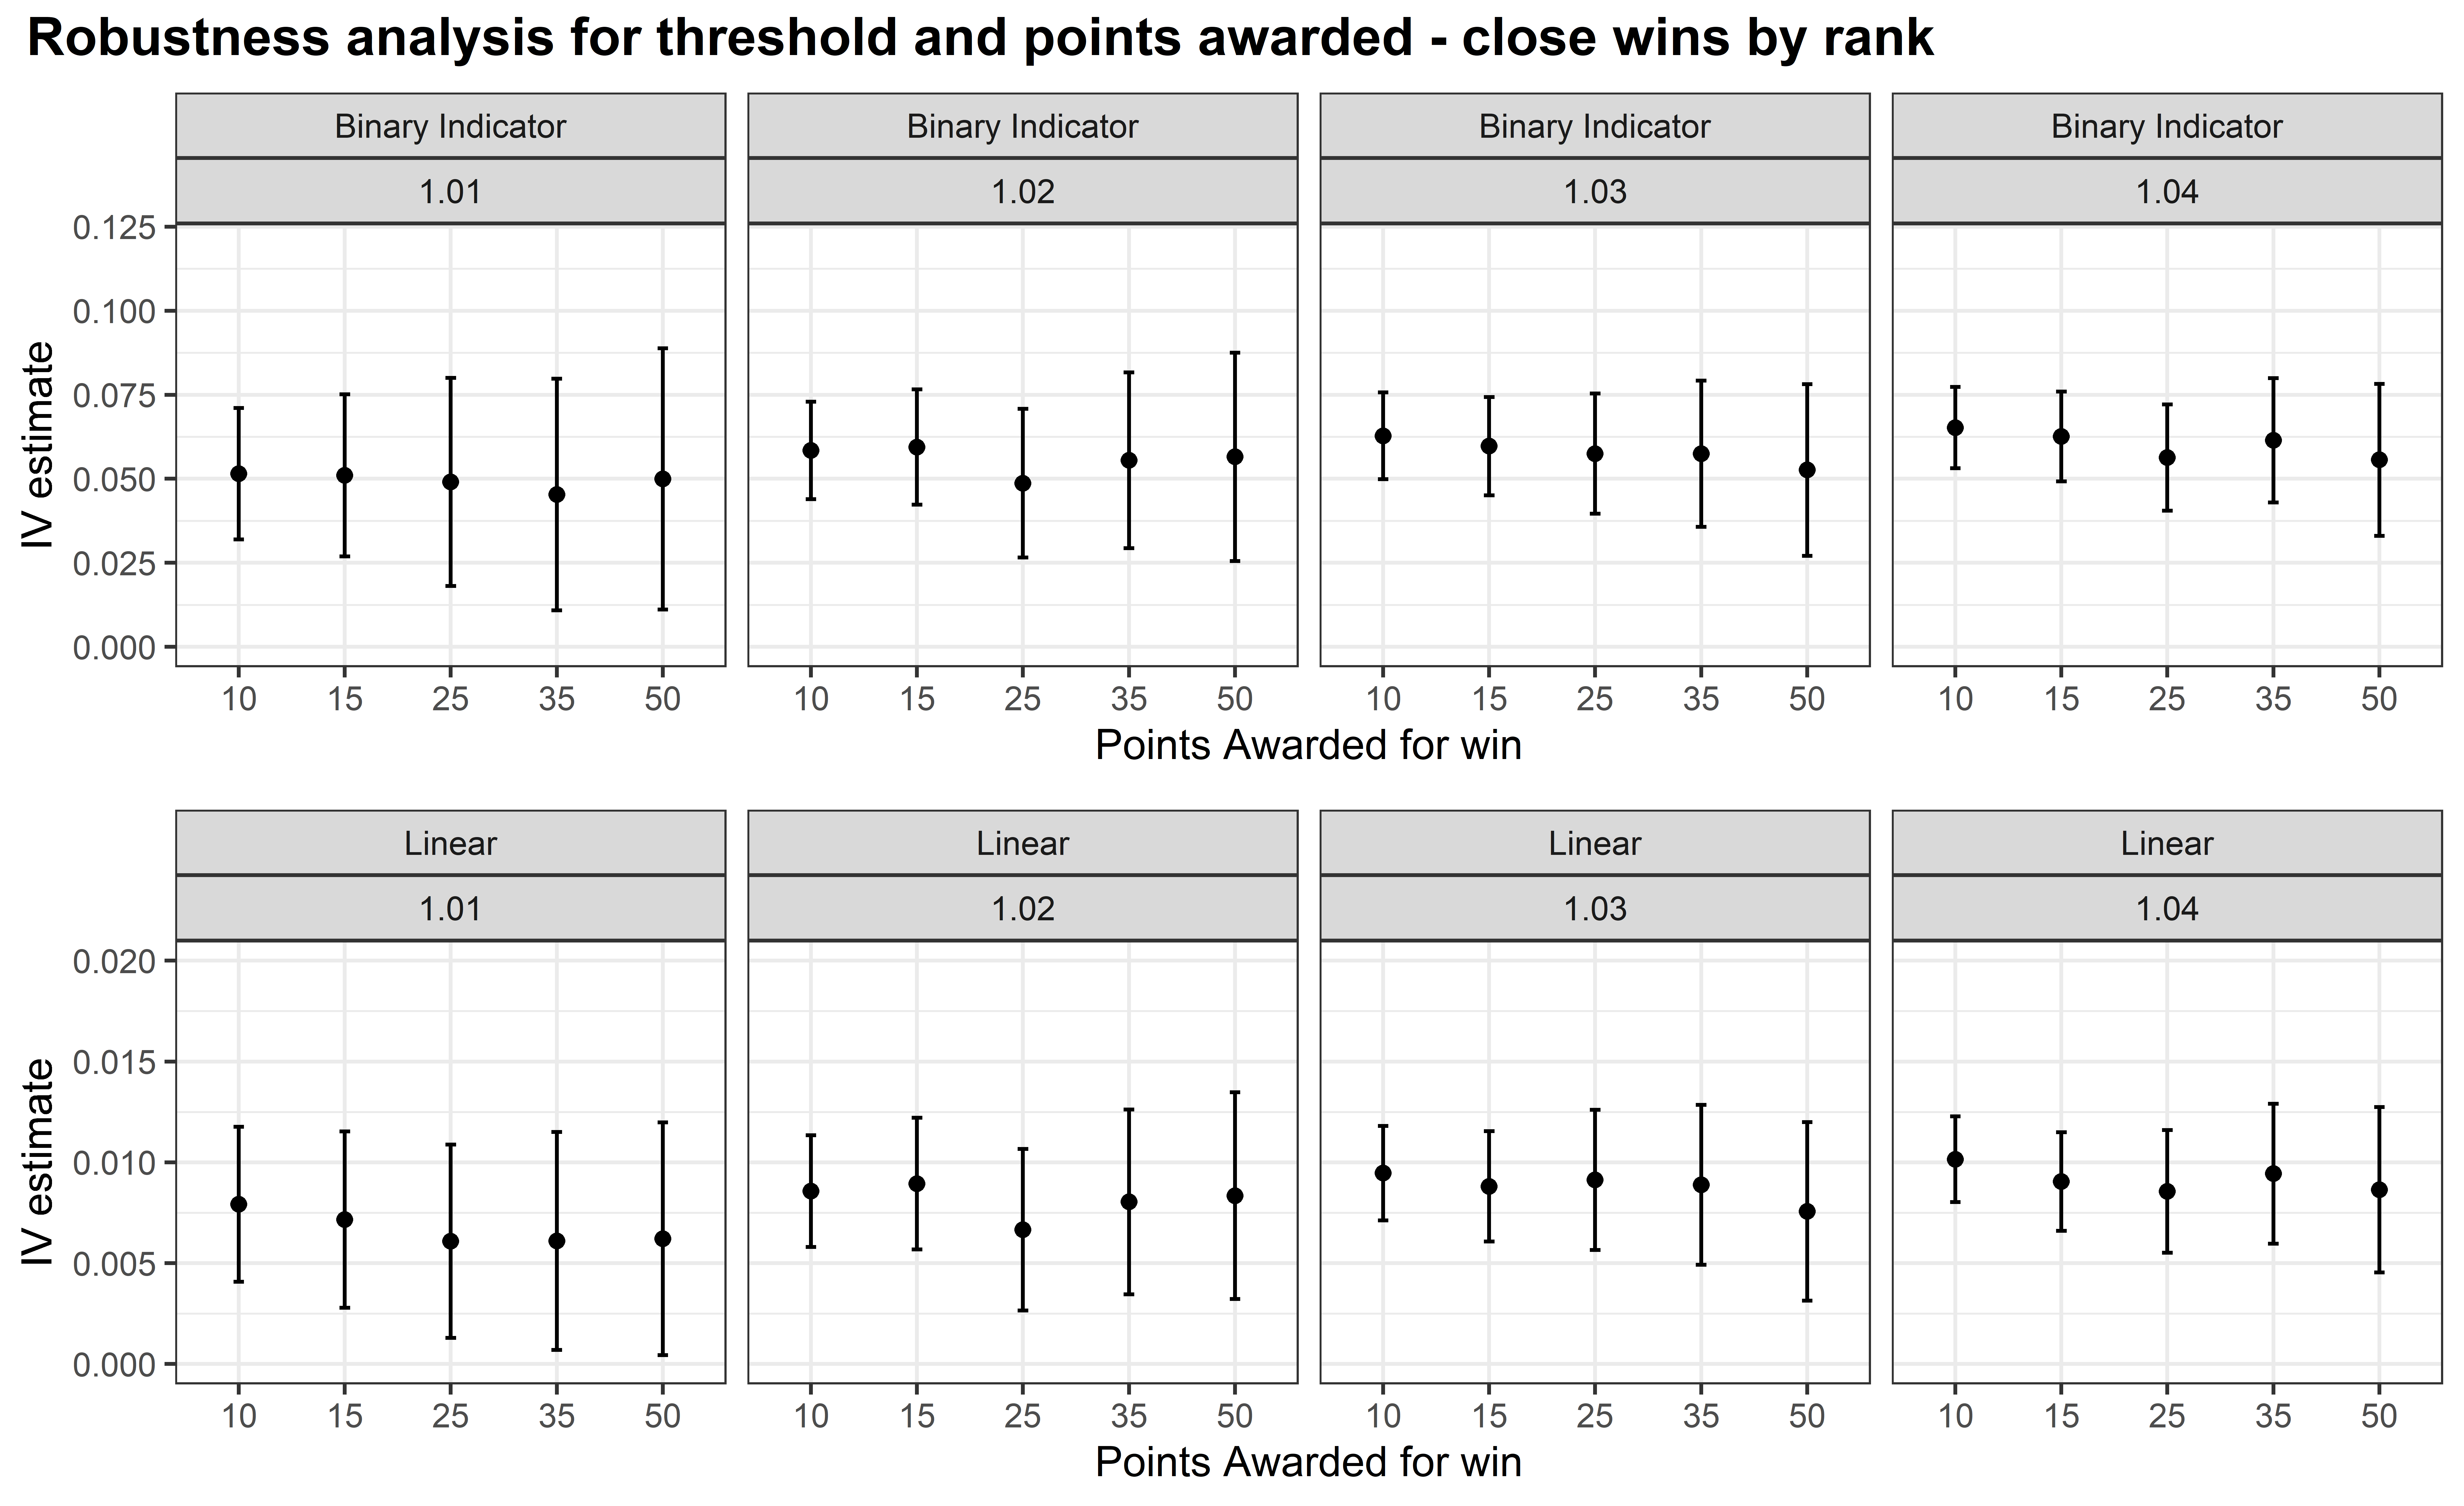
\includegraphics[scale=0.65]{plot_robustness_rank.png}
  \caption{Robustness analysis for parameters in the IV-Rank strategy}
  \label{fig:plot_robustness_rank}
\end{figure}
